\chapter[Referencial Teórico]{Referencial Teórico}

Neste capítulo, é apresentado os conceitos teóricos utilizados como base para o desenvolvimento do catálogo de segurança para o padrão arquitetural MVC. Antes de entender os conceitos relevantes para o desenvolvimento do catálogo é importante entender a definição de software, e segundo \cite{sommerville2003engenharia} pode ser entendido como programas de computador e toda documentação associada, e são produzidos através de uma disciplina da engenharia que preocupa com todos os aspectos da produção de software, essa disciplina é denominada de Engenharia de Software.

A figura \ref{BigPicture} apresenta a visão geral da construção do catálogo, partindo da Engenharia de Software e apoiando principalmente em duas disciplinas a  (i) Engenharia de Requisitos que compõe-se de um conjunto de tarefas e técnicas que auxiliam a promoção do entendimento dos requisitos, essa disciplina será detalhada na seção \ref{sec:requisitos} então entramos no contexto da orientação a meta que trata os requisitos funcionais e não funcionais como metas a serem alcançadas detalhado na subseção \ref{subsec:orientacaoMeta}, devido ao foco do trabalho ser os requisitos não funcionais (\ref{subsec:requisitosNaoFuncionais}) e utiliza-se o NFR \ref{sec:NFR} framework para tratar os requisitos não-funcionais, (ii) Desenho de software é a área da Engenharia de Software que possui como uma de suas preocupações o planejamento e a definição do padrão arquitetural a ser utilizado

\begin{figure}[h]
	\centering
	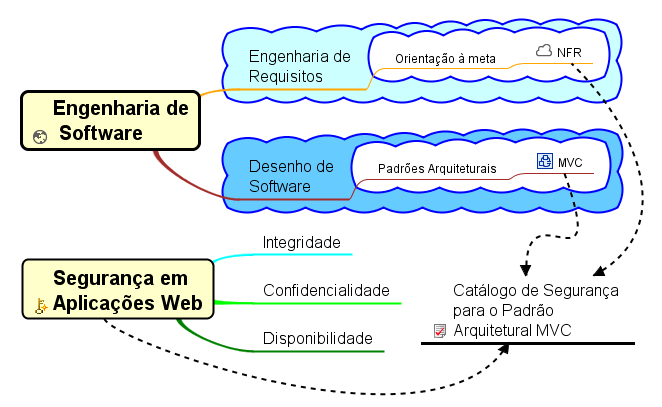
\includegraphics[keepaspectratio=true,scale=1.0]{figuras/bigPicture.png}
	\caption{Visão geral da proposta do catálogo.}
	\label{BigPicture}
\end{figure}



\section{Engenharia de Requisitos}
\label{sec:requisitos}

O conjunto de tarefas e técnicas utilizadas para promover o entendimento dos requisitos é denominado Engenharia de Requisitos. No desenvolvimento de software, pode ser vista como uma fase importante de Engenharia de Software que se inicia na atividade de comunicação e continua até a entrega do produto, sendo adaptada de acordo com as necessidades do processo de desenvolvimento, do produto e dos \textit{stakeholders} \cite{pressman2011engenharia}.

A Engenharia de Requisitos abrange sete fases distintas: concepção, levantamento, elaboração, negociação, especificação, verificação e validação \cite{pressman2011engenharia}. De acordo com \cite{kotonya1998requirements}, durante a execução das atividades das fases da Engenharia de Requisitos, alguns problemas são relatados como: (i) os requisitos não refletem as reais necessidades do cliente de acordo com o sistema a ser desenvolvido; (ii) são inconsistentes e/ou incompletos; (iii) é complexa a realização de alguma mudança no requisito, logo após terem sido acordados entre as partes; e (iv) comumente são interpretados de maneira errada pela equipe de desenvolvimento, diante do que foi solicitado pelo cliente. 


Boa parte dos modelos utilizados na Engenharia de Requisitos não possuem tratamento adequado para lidar com os critérios de qualidade. Logo, o tratamento desses atributos tem sido uma preocupação na comunidade da Engenharia de Requisitos. Esforços no sentido de aprimorar os modelos e especificações desses requisitos são fortemente associados à comunidade de pesquisadores da Engenharia de Requisitos Orientada a Meta (GORE) \cite{chung2012non}. Neste trabalho, é abordado o uso de uma notação específica, proposta por essa comunidade, no caso, trata-se do NFR \textit{framework} \cite{chung2012non}. 

O NFR \textit{framework} é um \textit{Framework} conceitual que procura lidar com os requisitos não funcionais, permitindo especificar os mesmos em um alto nível de abstração e, gradualmente, fornecendo insumos para que essa especificação seja trazida para um nível mais baixo de abstração. Nesse último nível, são especificadas as operacionalizações, as quais evidenciam alternativas para viabilizar a implementação desses requisitos no nível de código. Mais adiante, serão apresentados detalhes dessa notação.

\subsection{Engenharia de Requisitos Orientada à Meta}
\label{subsec:orientacaoMeta}

A Engenharia de Requisitos Orientada à Meta (GORE) tem-se popularizado nos últimos anos e constitui-se no tratamento dos requisitos funcionais e não funcionais como metas a serem alcançadas \cite{van2001goal}, pois seus modelos possuem como objetivo a modelagem da razão pela qual determinado requisito existe, essa modelagem promove ao engenheiro de requisitos uma estratégia mais detalhada do problema, podendo então encontrar uma solução mais adequada \cite{van2001goal}\cite{chung2012non}. O GORE é um paradigma que vem sendo cada vez mais reconhecido para a execução das atividades de elicitação, elaboração, análise, negociação, documentação e modificação dos requisitos de software\cite{van2001goal}.

Nas definições do GORE as metas são componentes essenciais, pois de acordo com \cite{van2001goal} uma meta é definida como propriedades do sistema que são expressas pelo \textit{stakeholders}, através de determinadas questões como o “\textbf{porquê}” uma meta é exigida, “\textbf{como}” ela pode ser atingida e quem será o responsável pela meta no sistema e no ambiente.

\begin{figure}[h]
	\centering
	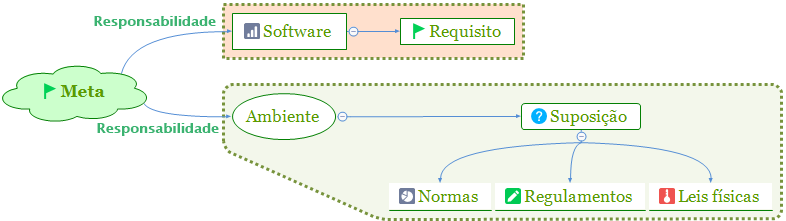
\includegraphics[keepaspectratio=true,scale=0.8]{figuras/GORE.png}
	\caption{Responsabilidades da meta sob o software e sob o ambiente.}
	\label{Gore}
\end{figure}

 Através da figura \ref{Gore} pode-se entender como são os comportamentos das metas no GORE. Representada pelo simbolo de uma nuvem uma meta, quando está sob a responsabilidade, de um único software essa meta pode-se tornar um requisito, de forma semelhante quando essa meta, está sob responsabilidade de um ambiente ela pode tornar-se uma suposição, diferente de um requisito as suposições não pode-ser aplicadas pelo software, mas podem ser satisfeitas devido as normas, regulamentos organizacionais e leis físicas \cite{van2001goal}. 


Existem diversos \textit{frameworks} orientados a metas como o NFR Framework \cite{chung2012non} e o i* \cite{istarwiki20}, esses \textit{frameworks} são detalhados nas seções \ref{sec:NFR} e \ref{sec:i*}, respectivamente

\subsection{Requisitos Não-Funcionais}
\label{subsec:requisitosNaoFuncionais}


\section{NFR Framework}
\label{sec:NFR}

O NFR \textit{Framework}  é um modelo intencional que ajuda desenvolvedores e engenheiros de requisitos a lidarem com requisitos não-funcionais, através de um grafo chamado de \textit{Softgoal Interdependency Graphs} (SIGs). Nesse grafo, os requisitos podem ser analisados, uma vez que o SIG permite uma visão vertical desde a estratégia de alto nível até os detalhes operacionais;  possuindo operadores lógicos AND (E) e OR (OU) que promovem uma melhor tomada de decisão; onde  os requisitos não funcionais são escritos através de uma notação formal que permite provar a sua correção e completude. O framework também possui uma estrutura que pode ser orientada por processo, dando suporte às atividades do processo de engenharia de requisitos, e pode ser utilizado como complemento nas abordagens tradicionais de desenvolvimento de software \cite{chung2012non}.

O NFR Framework utiliza o conceito de metas flexíveis que é uma condição ou um estado no mundo real que deseja ser alcançado, podendo assumir natureza subjetiva, pois o RNF pode variar de acordo com o julgamento de cada pessoa; e natureza relativa, pois o RNF pode depender de algum tipo de relação com outro RNF.  A notação no SIG para a \textbf{meta flexível} é um símbolo similar ao de uma nuvem, conforme mostra a figura \ref{fig01}. Esse, com pequenas variações na forma, pode representar uma \textbf{operacionalização} (nuvem em negrito), e também uma \textbf{reivindicação} (nuvem tracejada).

\begin{figure}[h]
	\centering
	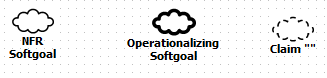
\includegraphics[keepaspectratio=true,scale=0.9]{figuras/tiposDeSoftgoals.png}
	\caption{Representação gráfica dos tipos de metas flexíveis.}
	\label{fig01}
\end{figure} 

Para facilitar o entendimento das decisões tomadas, a meta flexível possui \textit{labels} que determinam o grau em que determinado RNF é satisfeito, de acordo com um conjunto de decisões do projeto. Essas labels são: satisfeita, fracamente satisfeita,  negada, fracamente negada, indecidida e crítica \cite{chung2012non}. Outra notação importante é o grau de prioridade de uma meta flexível, representado por “\textbf{!}” ou “\textbf{!!}” para um grau de prioridade maior.

\begin{figure}[h]
	\centering
	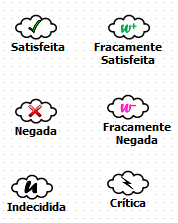
\includegraphics[keepaspectratio=true,scale=0.9]{figuras/labelsSoftgoals.png}
	\caption{Representação gráfica das labels das metas flexíveis.}
	\label{fig02}
\end{figure} 

As relações que as metas flexíveis possuem uma com as outras é estabelecida através de interdependências, sendo essas as que realizam o registro do refinamento das metas flexíveis em metas flexíveis mais específicas (filhos) De certa forma, tal detalhamento em outras metas, contribui para satisfazer a meta flexível mais genérica (pai). Os tipos de contribuições são apresentados na tabela \ref{tiposDeContribuições} adaptado de  \cite{chung2012non}.

\begin{table}[h!]
	\centering
	\caption{Tipos de contribuições.}
	\label{tiposDeContribuições}
	\begin{tabular}{|l|l|}
		\hline
		\textbf{Símbolo} & \textbf{Descrição} \\ \hline
		\multirow{2}{*}{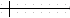
\includegraphics[scale=0.9]{figuras/And.png}} & \multirow{2}{*}{AND: Se todos os filhos são satisfeitos o pai também será satisfeito.} \\
		&  \\ \hline
		\multirow{2}{*}{\includegraphics[scale=0.9]{figuras/OR.png}} & \multirow{2}{*}{OR: Se qualquer filho é satisfeito o pai também será satisfeito.} \\
		&  \\ \hline
		\multirow{2}{*}{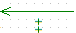
\includegraphics[scale=0.9]{figuras/Make.png}} & \multirow{2}{*}{\begin{tabular}[c]{@{}l@{}}MAKE: Pode ser tratado de forma semelhante ao AND, pois se \\ o filho for satisfeito o pai pode ser satisfeito.\end{tabular}} \\
		&  \\ \hline
		\multirow{2}{*}{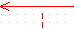
\includegraphics[scale=0.9]{figuras/Break.png}} & \multirow{2}{*}{\begin{tabular}[c]{@{}l@{}}BREAK: Fornece apoio negativo, pois se o filho é satisfeito o \\ pai pode ser negado.\end{tabular}} \\
		&  \\ \hline
		\multirow{2}{*}{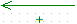
\includegraphics[scale=0.9]{figuras/Help.png}} & \multirow{2}{*}{HELP: Se todos os filhos são satisfeitos o pai também será satisfeito.} \\
		&  \\ \hline
		\multirow{2}{*}{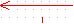
\includegraphics[scale=0.9]{figuras/Hurt.png}} & \multirow{2}{*}{HURT: Se todos os filhos são satisfeitos o pai será fracamente negado.} \\
		&  \\ \hline
		\multirow{2}{*}{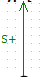
\includegraphics[scale=0.9]{figuras/SomeMais.png}} & \multirow{2}{*}{SOME+: Representa a existência de alguma contribuição positiva.} \\
		&  \\ \hline
		\multirow{2}{*}{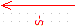
\includegraphics[scale=0.9]{figuras/SomeMenos.png}} & \multirow{2}{*}{SOME-: Representa a existência de alguma contribuição negativa.} \\
		&  \\ \hline
	\end{tabular}
\end{table}

A figura \ref{exemploNFR} apresenta uma decomposição de uma meta flexível em outras metas de mesma natureza. Consideramos, nesse exemplo, o RNF: “manter as contas com boa segurança”. Usando a notação do NFR \textit{Framework}, representou-se a meta flexível  “segurança de contas”, no nível mais generalista do grafo. Em segundo nível, são especificadas as principais metas flexíveis que merecem ser consideradas para que a meta generalista seja "satisfeita", no caso: “Integridade de contas”, “Confidencialidade de contas” e “Disponibilidade de contas” \cite{chung2012non}.

\pagebreak

\begin{figure}[h!]
	\centering
	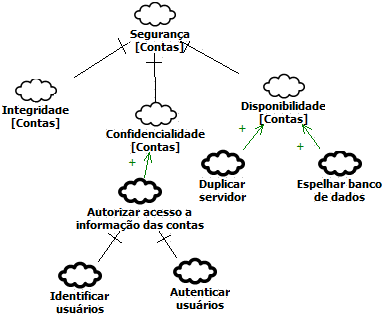
\includegraphics[keepaspectratio=true,scale=1.0]{figuras/exemploNFR.png}
	\caption{Operacionalização de segurança de contas. Adapatado de \cite{chung2012non}, \cite{affleck2012supporting}.}
	\label{exemploNFR}
\end{figure} 

Confidencialidade de contas é operacionalizada em “Autorizar acesso à informação das contas”, que possui uma contribuição do tipo HELP com seu pai. Dada a relação do tipo AND, entre essa operacionalização e as operacionalizações "Identificar usuários" e "Autenticar usuários", tem-se que a operacionalização "Autorizar acesso à informação das contas"  será realizada se ambas as operacionalizações, "Identificar usuários" e "Autenticar usuários", forem realizadas. Supondo que tudo tenha sido realizado com sucesso, tem-se que esse processo de operacionalização contribui positivamente - HELP (AJUDA) - a atingir "Confiabilidade de contas". Como essa meta flexível está especificada em uma relação de AND com as metas flexíveis "Integridade de contas" e "Disponibilidade de contas", pode-se dizer que em termos de "Confiabilidade de contas", "Segurança de contas" tem a ser "satisfeita". Mas, resta ainda ponderar se "Integridade de contas" e "Disponibilidade de contas" serão de fato "satisfeitas". O modelo, da forma como está especificado, não permite avaliar tais aspectos, visto que representa apenas uma visão parcial dessas metas flexíveis.


Para Disponibilidade de contas a mesma é operacionalizada em “Duplicar servidor” e “Espelhar banco de dados” essas operacionalizações possuem contribuições do tipo HELP e mesmo pai, e para a meta flexível ser satisfeita, ambas as operacionalizações devem ser satisfeitas \cite{affleck2012supporting}. 


\section{i*}
\label{sec:i*}

\section{FURPS}


\section{Arquitetura de Software}
\label{sec:arquitetura}
\subsection{MVC - Model-View-Controller}
\label{subsec:mvc}

\section{Segurança de Software}

\chapter{Suporte Tecnológico}

\chapter{Metodologia}
